% Source-page vector redraw from 2005 Spring Beijing Science, printed p. 213, Q12.
% Kept as a separate source-specific file. Dashed edges follow the visible source line styles.
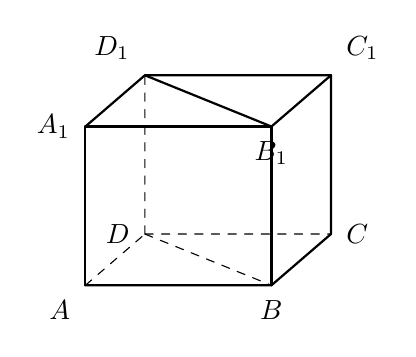
\begin{tikzpicture}[line cap=round, line join=round, scale=1.05]
\coordinate (A) at (0,0); \coordinate (B) at (2.25,0);
\coordinate (D) at (.72,.62); \coordinate (C) at (2.97,.62);
\coordinate (A1) at (0,1.92); \coordinate (B1) at (2.25,1.92);
\coordinate (D1) at (.72,2.54); \coordinate (C1) at (2.97,2.54);
% Solid visible cube edges
\draw[thick] (A)--(B)--(C);
\draw[thick] (A)--(A1)--(B1)--(B);
\draw[thick] (B1)--(C1)--(C);
\draw[thick] (A1)--(D1)--(C1);
\draw[thick] (C)--(C1);
% Hidden cube edges and hidden diagonal of BB1D1D
\draw[dashed] (A)--(D) (D)--(C) (D)--(D1);
\draw[dashed] (D)--(B);
% Visible diagonal of BB1D1D
\draw[thick] (D1)--(B1);
\node[below left=2pt] at (A) {$A$};
\node[below=2pt] at (B) {$B$};
\node[right=2pt] at (C) {$C$};
\node[left=2pt] at (D) {$D$};
\node[left=2pt] at (A1) {$A_1$};
\node[below=2pt] at (B1) {$B_1$};
\node[above left=2pt] at (D1) {$D_1$};
\node[above right=2pt] at (C1) {$C_1$};
\end{tikzpicture}
